\documentclass[a4paper,14pt]{extreport} % формат документа

\usepackage{amsmath}
\usepackage{cmap} % поиск в ПДФ
\usepackage[T2A]{fontenc} % кодировка
\usepackage[utf8]{inputenc} % кодировка исходного текста
\usepackage[english,russian]{babel} % локализация и переносы
\usepackage[left = 2cm, right = 1cm, top = 2cm, bottom = 2 cm]{geometry} % поля
\usepackage{listings}
\usepackage{graphicx} % для вставки рисунков
\usepackage{amsmath}
\usepackage{float}
\usepackage{multirow}
\graphicspath{{img/}}
\DeclareGraphicsExtensions{.pdf,.png,.jpg}
\newcommand{\anonsection}[1]{\section*{#1}\addcontentsline{toc}{section}{#1}}

\lstset{ %
	language=Lisp,                % Язык программирования 
	numbers=left,                   % С какой стороны нумеровать          
	frame=single,                    % Добавить рамку
}

\begin{document}
\begin{titlepage}

    \begin{table}[H]
        \centering
        \footnotesize
        \begin{tabular}{cc}
            \multirow{8}{*}{
\includegraphics[scale=0.35]{bmstu.jpg}}
            & \\
            & \\
            & \textbf{Министерство науки и высшего образования Российской Федерации} \\
            & \textbf{Федеральное государственное бюджетное образовательное учреждение} \\
            & \textbf{высшего образования} \\
            & \textbf{<<Московский государственный технический} \\
            & \textbf{университет имени Н.Э. Баумана>>} \\
            & \textbf{(МГТУ им. Н.Э. Баумана)} \\
        \end{tabular}
    \end{table}

    \vspace{-2.5cm}

    \begin{flushleft}
        \rule[-1cm]{\textwidth}{3pt}
        \rule{\textwidth}{1pt}
    \end{flushleft}

    \begin{flushleft}
        \small
        ФАКУЛЬТЕТ
        \underline{<<Информатика и системы управления>>\ \ \ \ \ \ \ 
        \ \ \ \ \ \ \ \ \ \ \ \ \ \ \ \ \ \ \ \ \ \ \ \ \ \ \ \ \ \ \ 
    \ \ \ \ \ \ \ \ \ \ \ \ \ \ \ } \\
        КАФЕДРА
        \underline{<<Программное обеспечение ЭВМ и
        информационные технологии>>
        \ \ \ \ \ \ \ \ \ \ \ \ \ \ \ \ \ \ \ \ }
    \end{flushleft}

    \vspace{2cm}

    \begin{center}
        \textbf{Рубежный контроль 1} \\
        \vspace{0.5cm}
    \end{center}

    \vspace{4cm}

    \begin{flushleft}
        \begin{tabular}{ll}
            \textbf{Дисциплина} & Экономика программной инженерии.  \\
            \\
            \textbf{Студент} & Сиденко А.Г. \\
             \textbf{Вариант} & 1 \\
            \textbf{Группа} & ИУ7-83Б \\
            \textbf{Оценка (баллы)} & \\
            \textbf{Преподаватель} & Барышникова М.Ю., Силантьева А.В.   \\
        \end{tabular}
    \end{flushleft}

    \vspace{4cm}

   \begin{center}
        Москва, 2021 г.
    \end{center}

\end{titlepage}

\begin{enumerate}

\item \textbf{Описание проекта}
Группа из 7 человек, длительность не более 3 мес., бюджет не более 650 тыс. руб.

Команда начинающих разработчиов во главе с опытным ведущим программистом ориентирована на создание собственной Интернет-компании с <<нуля>>. Проект предусматривает подготовительные работы по обучению персонала созданиям web-сайтов и разработке представительских и корпоративного сайтов, необходимых для организации коммерческой деятельности по получению заказов на Интернет-продукты.

\item \textbf{Задание 1}

Настройка рабочей среды проекта

\begin{figure}[H]
  \centering
  \caption{Настройка параметров проекта. }
  
\includegraphics[scale=0.5]{1}
\end{figure}

\begin{figure}[H]
  \centering
  \caption{Устанавливаем дату начала. }
  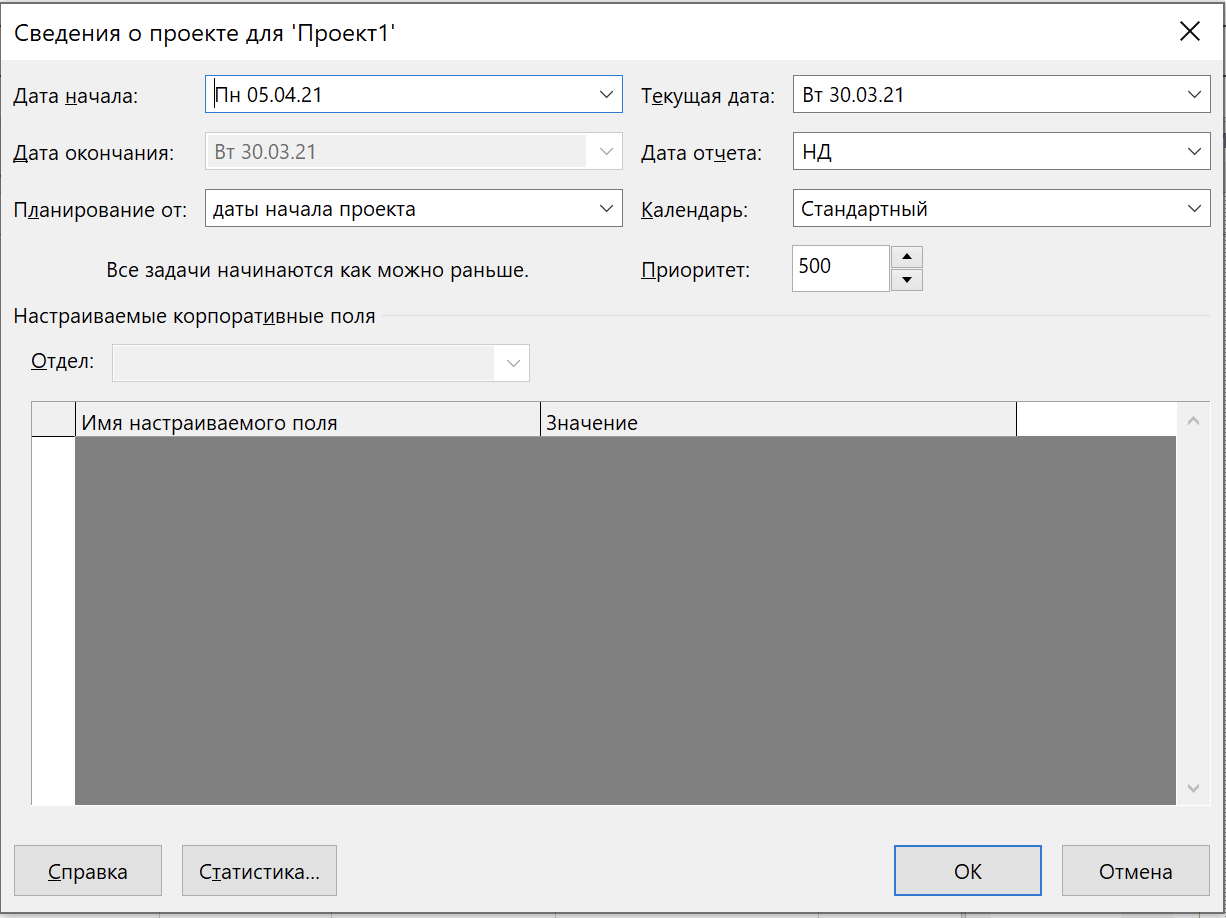
\includegraphics[scale=0.6]{2}
\end{figure}

\begin{figure}[H]
  \centering
  \caption{Настройка календаря. }
  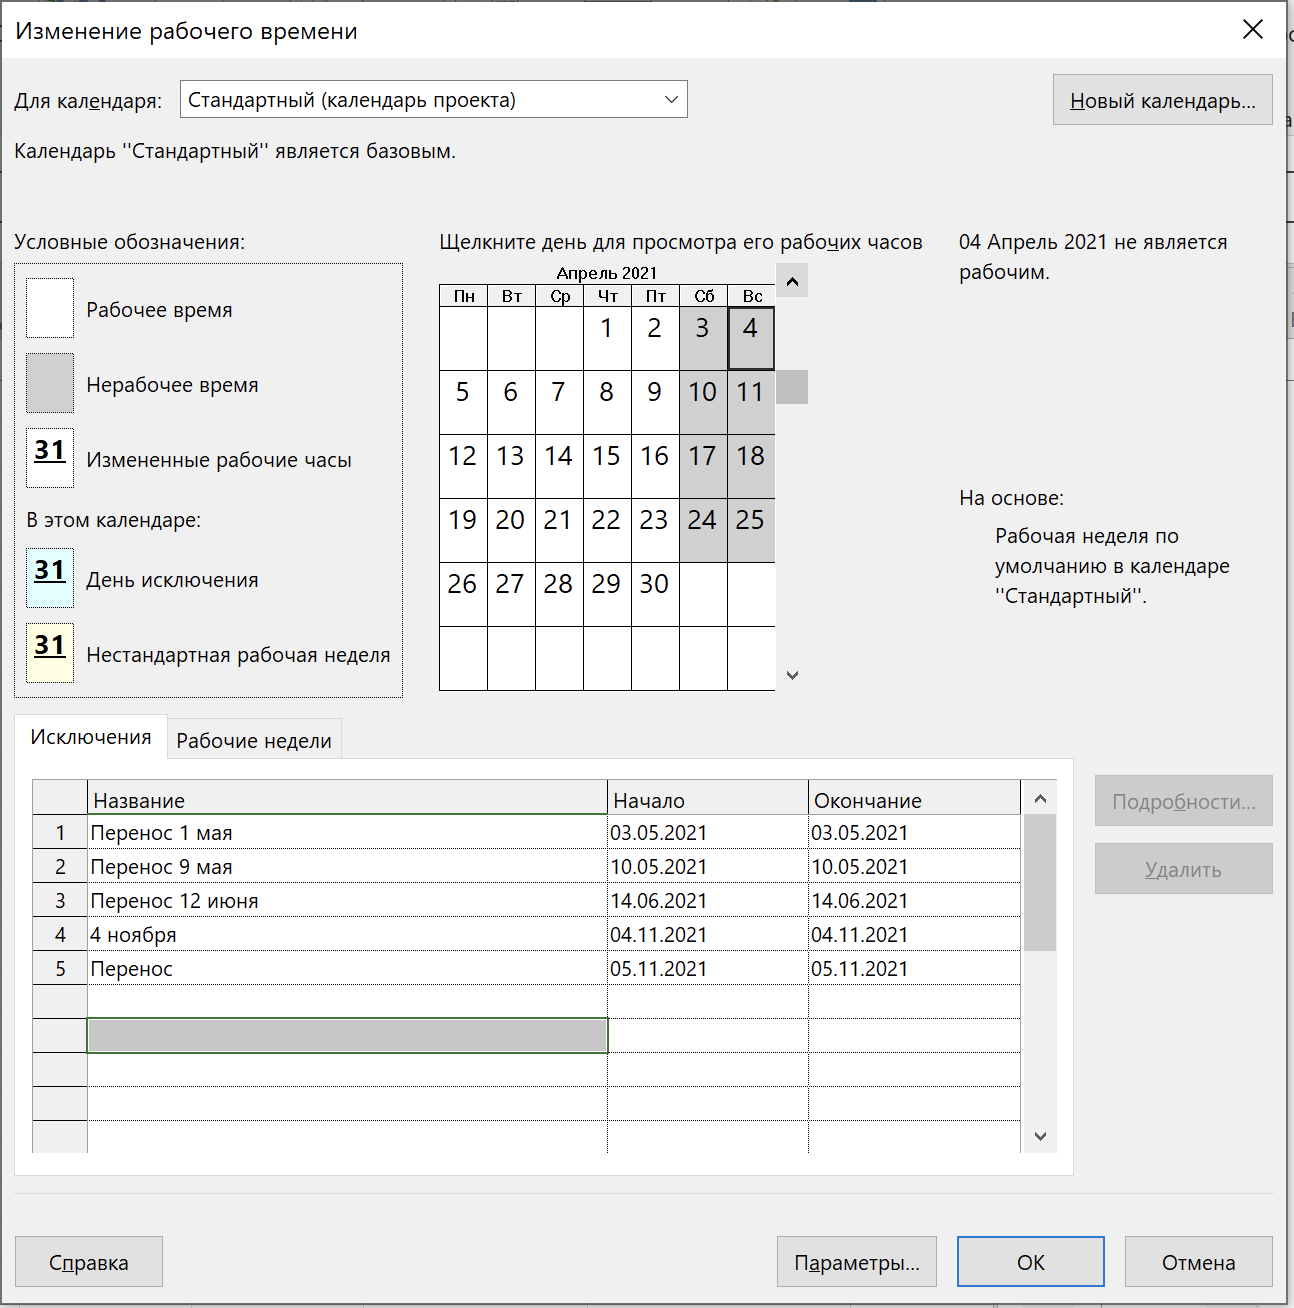
\includegraphics[scale=0.6]{3}
\end{figure}

\item \textbf{Задание 2}

Вводим список задач

\begin{figure}[H]
  \centering
  \caption{Список задач проекта. }
  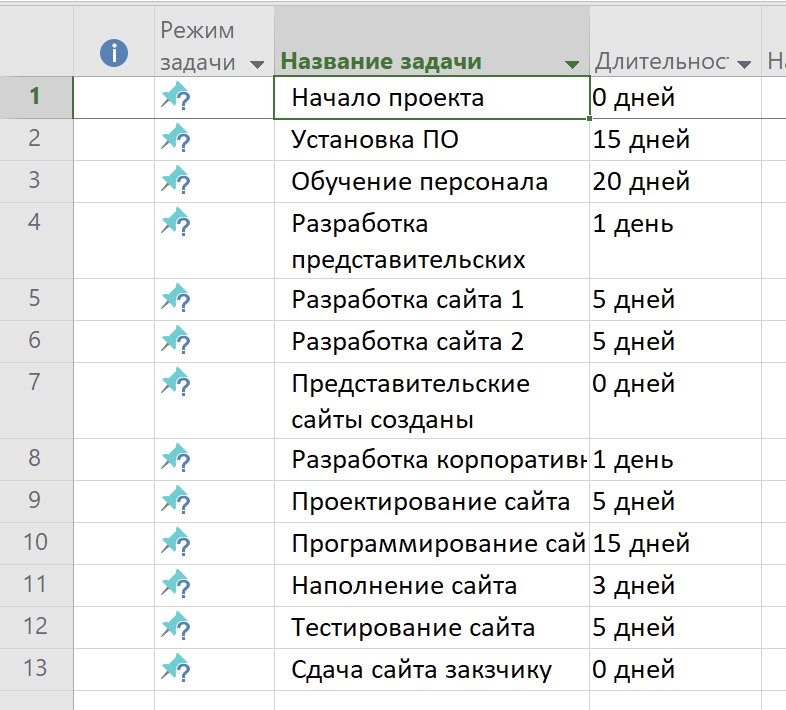
\includegraphics[scale=0.6]{4}
\end{figure}

\item \textbf{Задание 3}

Структурируем список задач

\begin{figure}[H]
  \centering
  \caption{Структурированный список задач проекта. }
  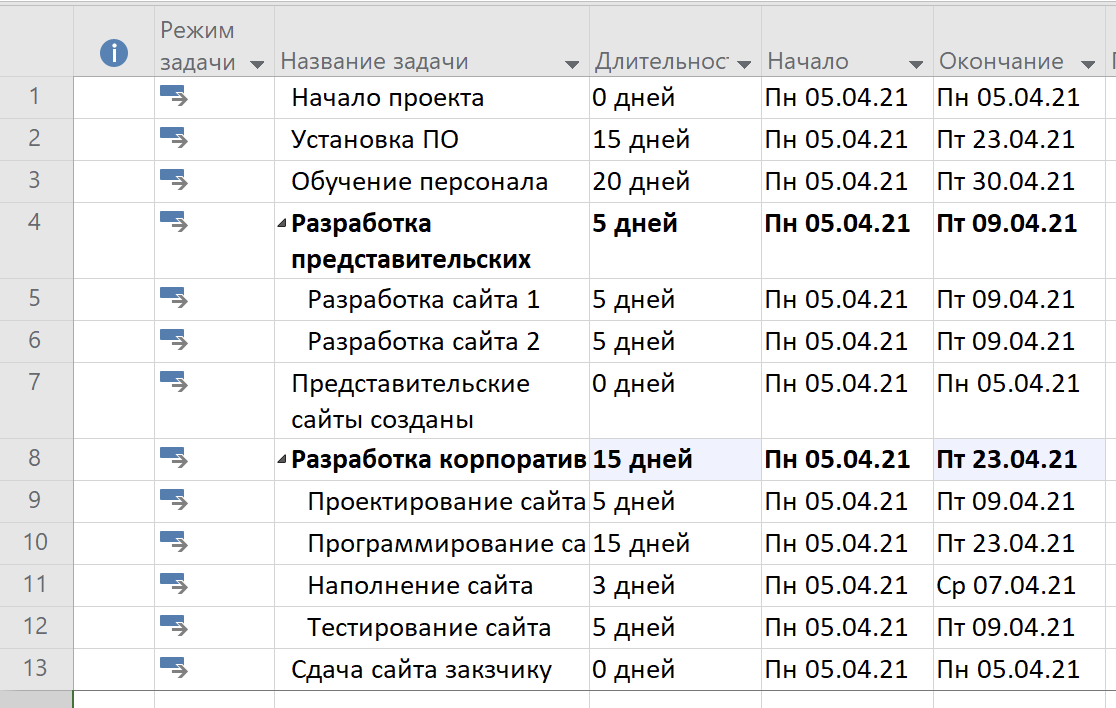
\includegraphics[scale=0.6]{5}
\end{figure}

\item \textbf{Задание 4}

Создаем связи между задачами

\begin{figure}[H]
  \centering
  \caption{Структурированный список задач проекта со связями. }
  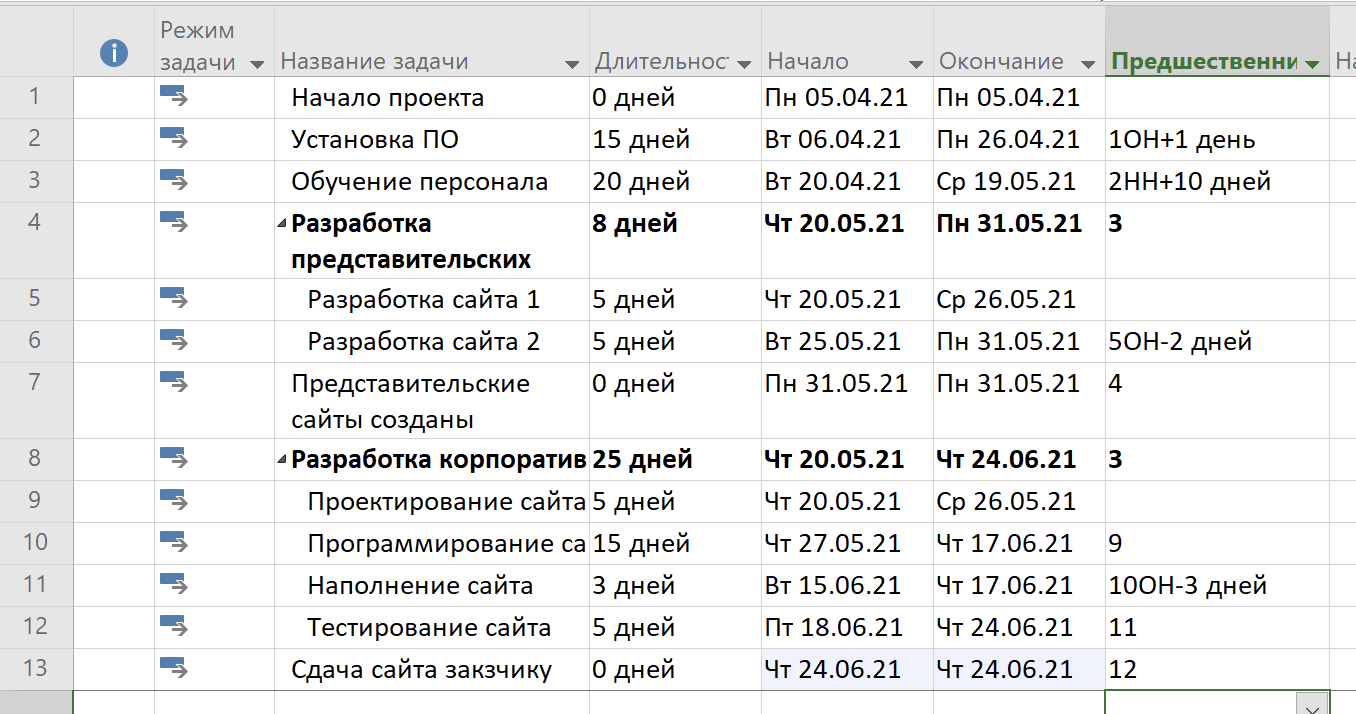
\includegraphics[scale=0.6]{6}
\end{figure}

\item \textbf{Задание 5}

Создаем список ресурсов. Добавляем заметки Соколову и Петрову. Также задаем расход бумаги -- 3 пачки в месяц (для этого добавляем суммарную задачу) и назначаем ресурс на нее.

\begin{figure}[H]
  \centering
  \caption{Список ресурсов. }
  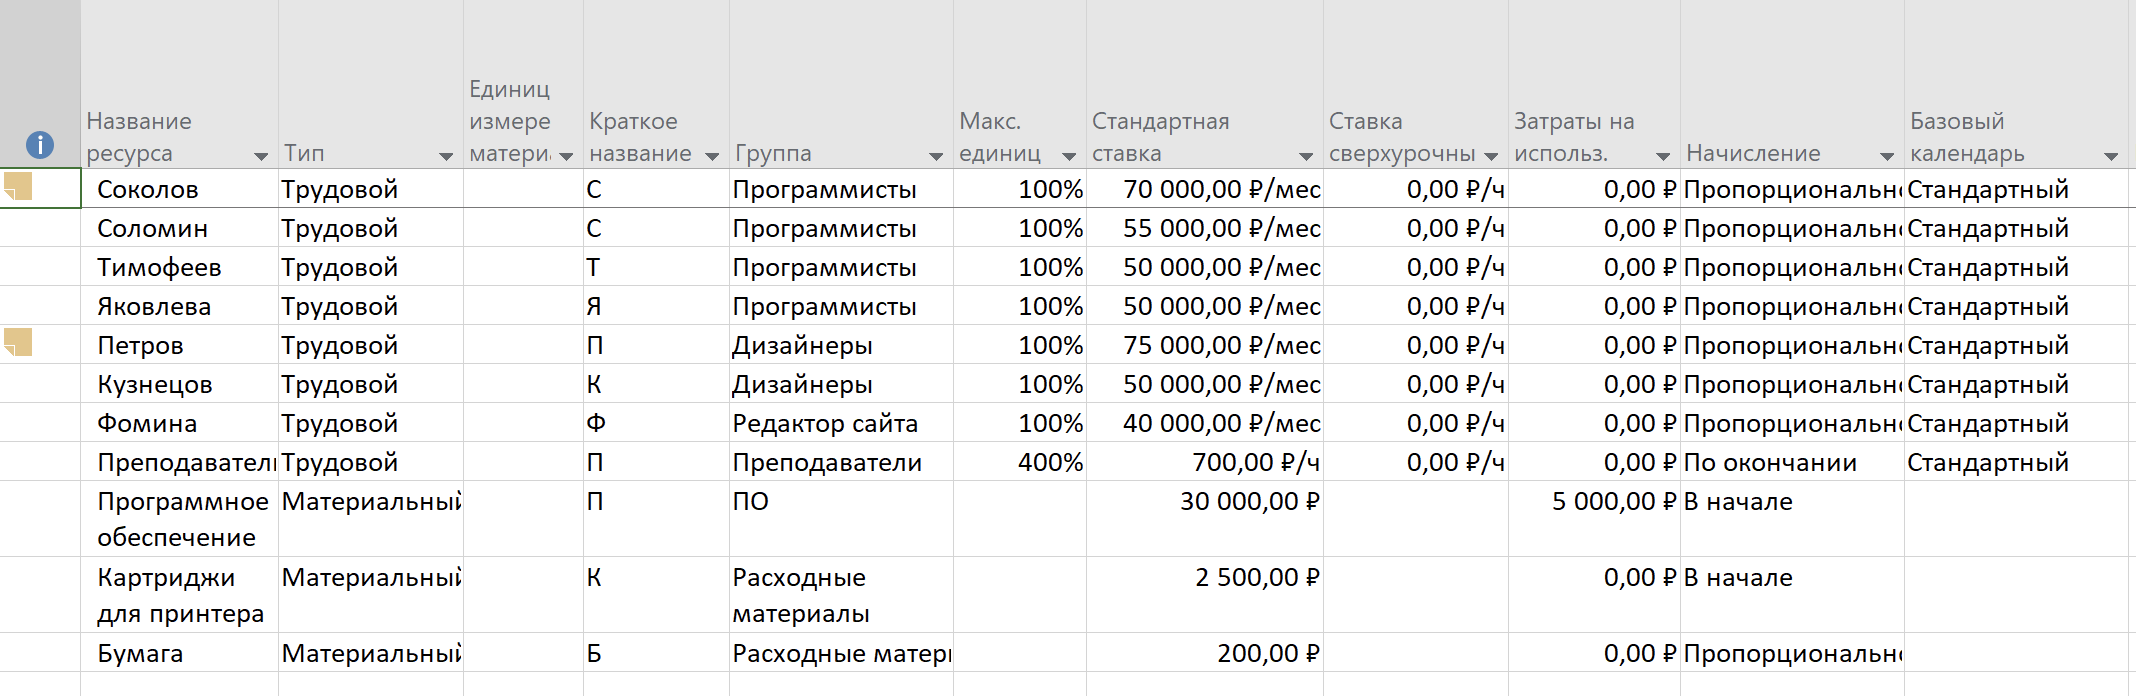
\includegraphics[scale=0.5]{7}
\end{figure}

\begin{figure}[H]
  \centering
  \caption{Расход бумаги. }
  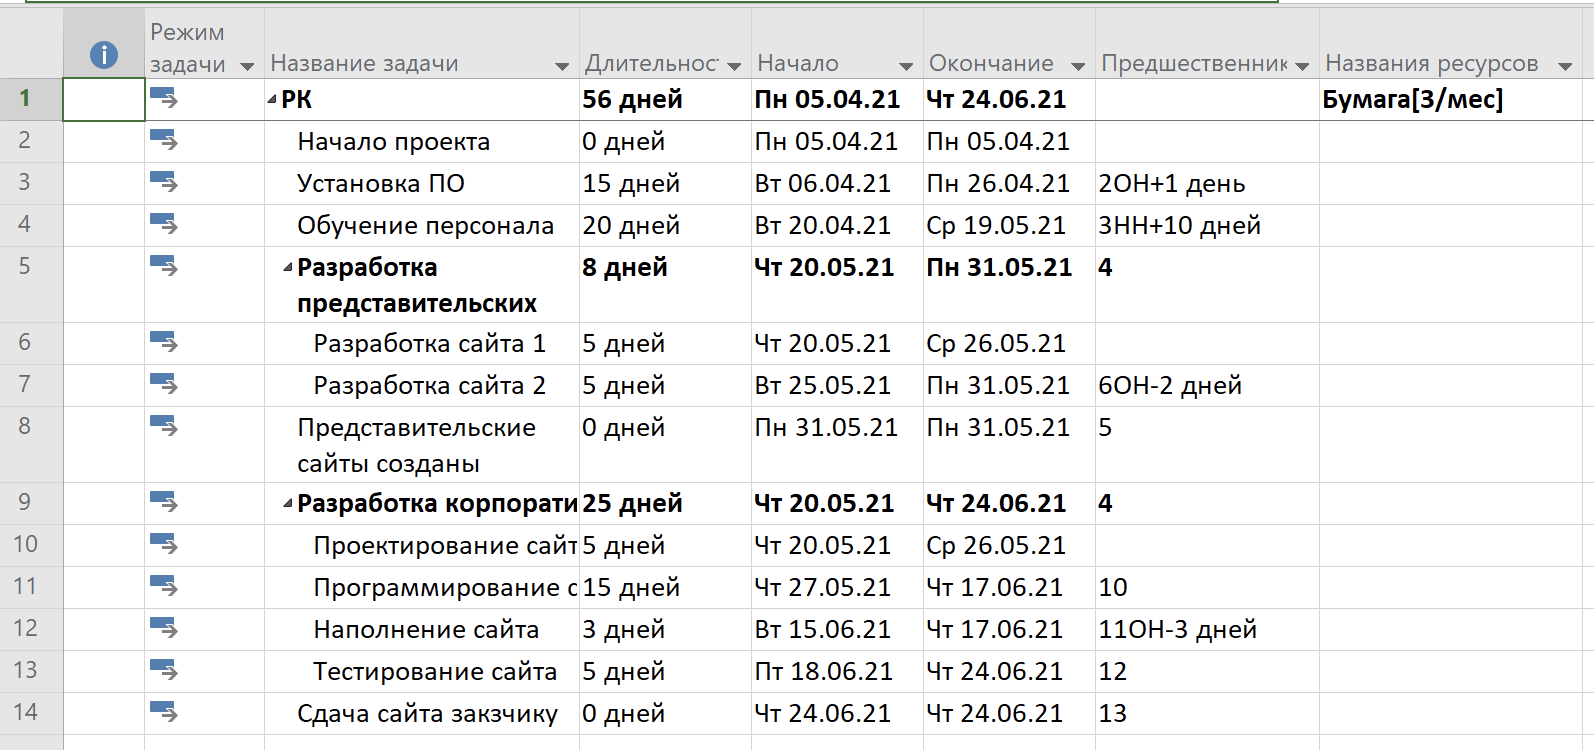
\includegraphics[scale=0.5]{8}
\end{figure}

И назначаем ресурсы на задачи и задаем фиксированные.

\begin{figure}[H]
  \centering
  \caption{Итог. }
  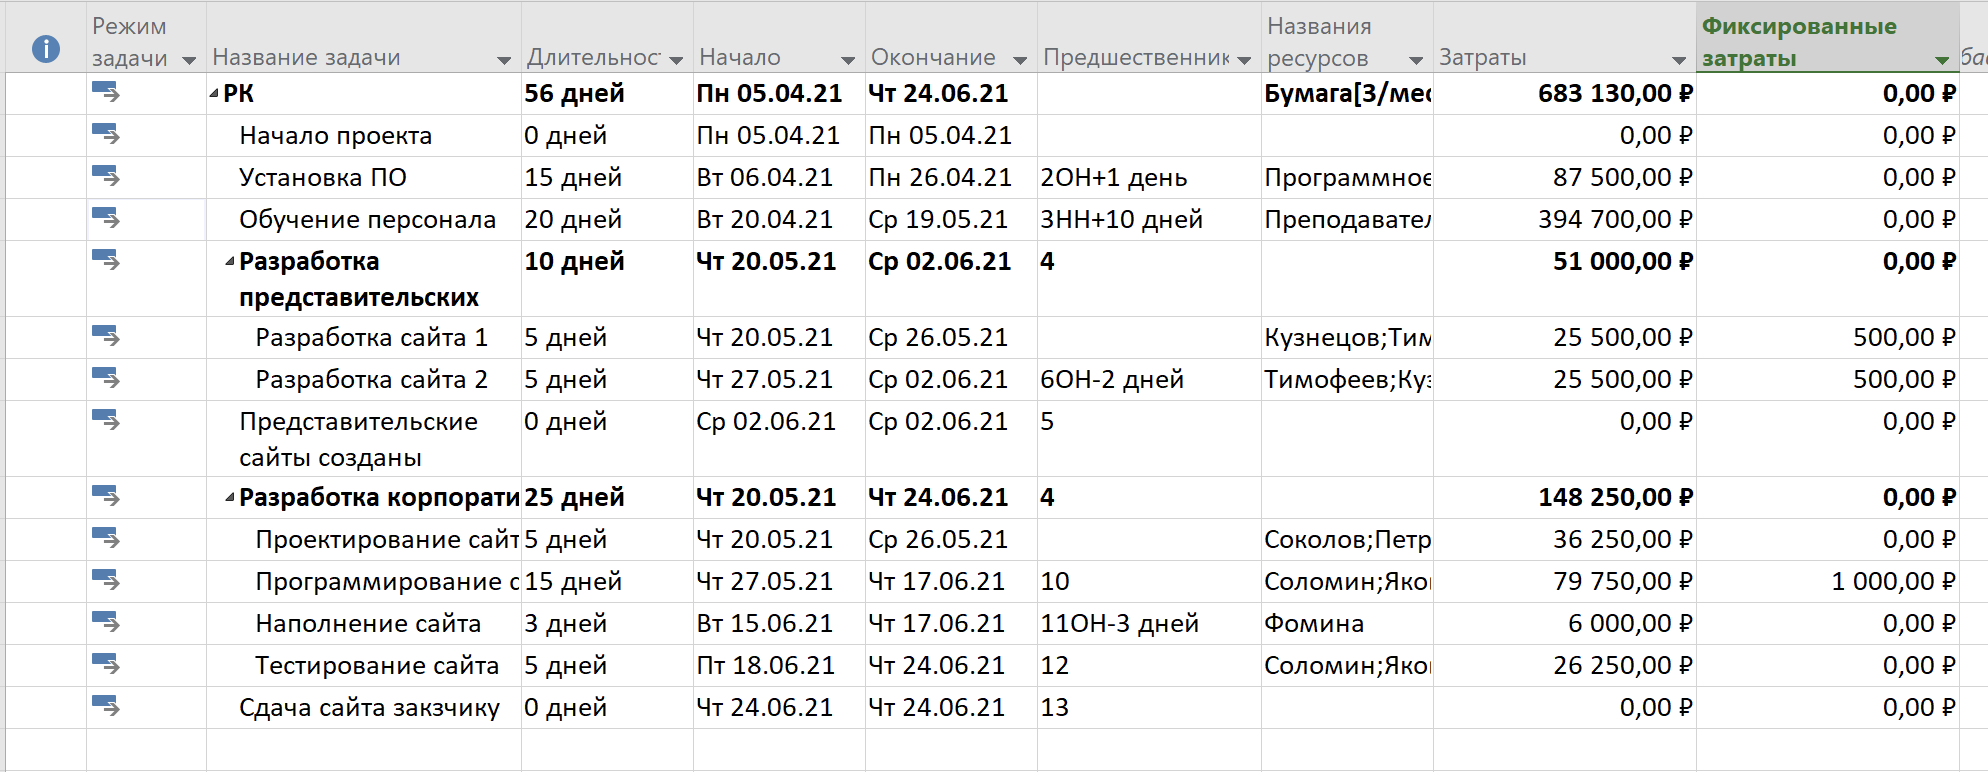
\includegraphics[scale=0.5]{9}
\end{figure}

В результате после назначения ресурсов задачам, срок выполнения работ 24.06.2021, а затраты – 683130 рублей.

\item \textbf{Задание 7}

Разбиваем задачу на подзадачи, длительностью 2 и 3 дня соответственно и назначить разработку дизайна сайта Кузнецову, а программирование сайта -- Тимофееву. Устанавливаем новые связи

\begin{figure}[H]
  \centering
  \caption{Разбиваем задачу на подзадачи. }
  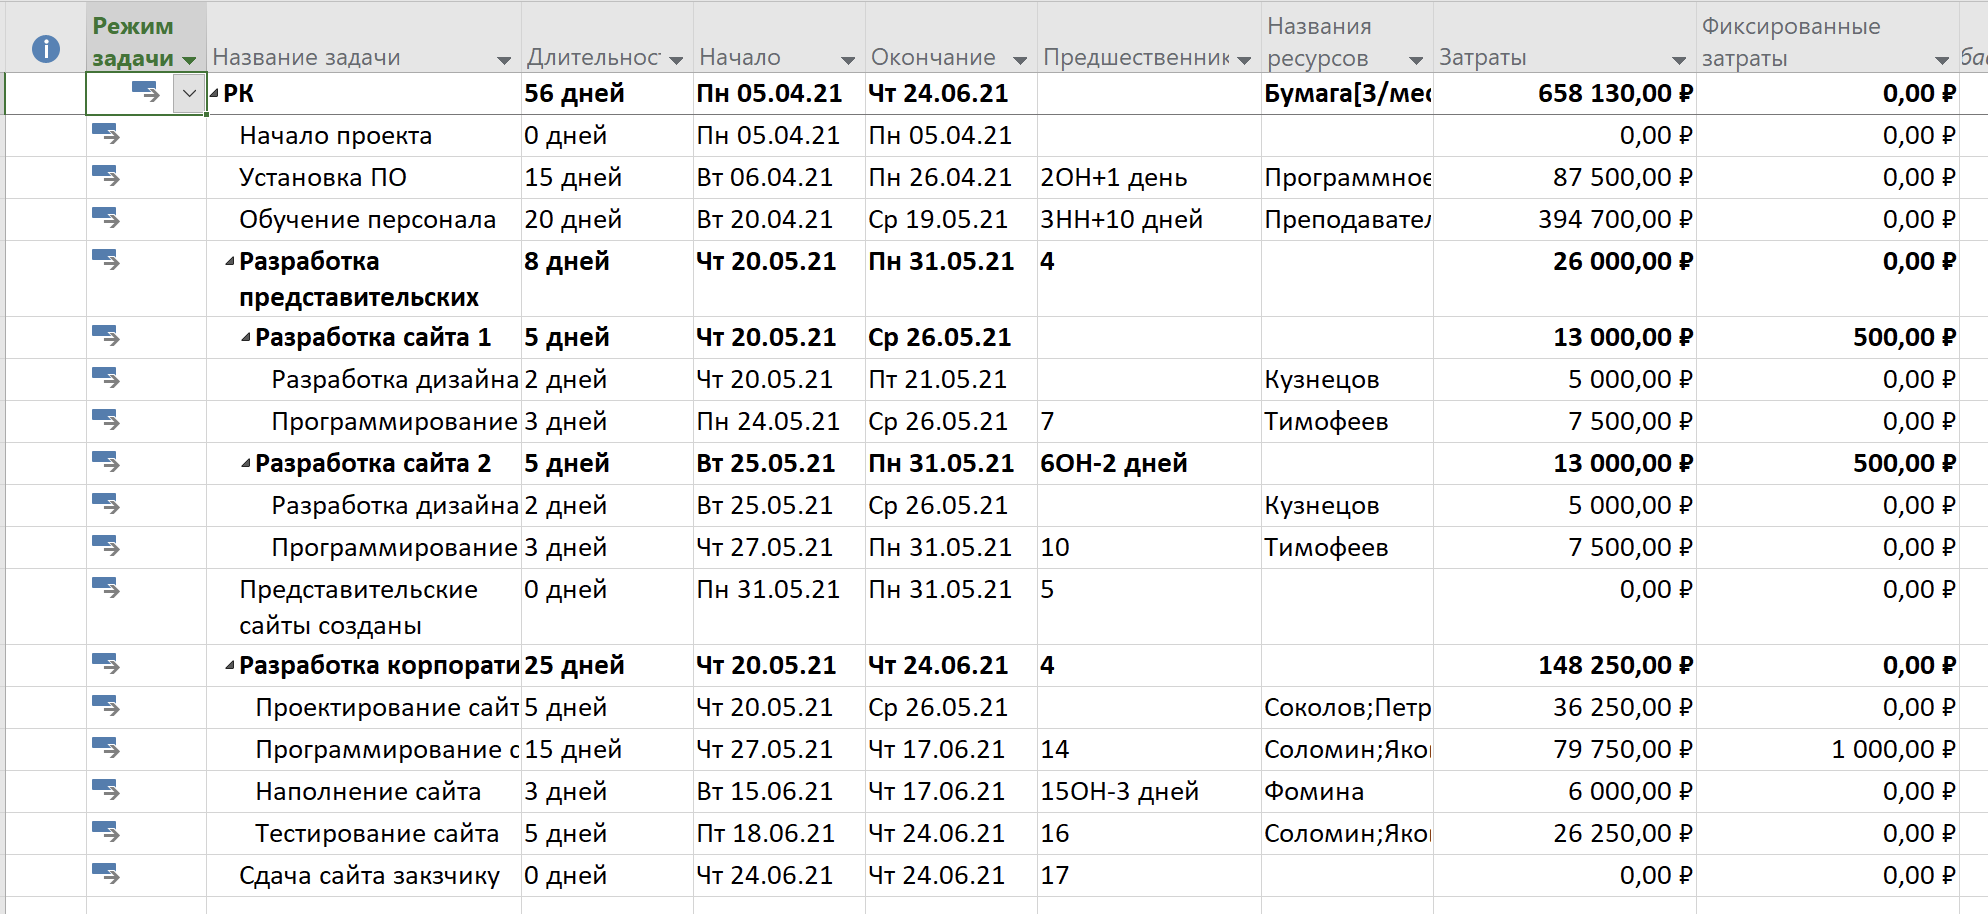
\includegraphics[scale=0.6]{10}
\end{figure}

После разбиения задачи, на подзадачи, их выполнение могло быть распараллелено (Тимофеев разрабатывал сайт 1, Кузнецов уже разрабатывал дизайн сайта 2), уменьшились трудозатраты и соответственно стоимость проекта до 658130.

\item \textbf{Задание 8}

Переназначение ресурсов.

\begin{figure}[H]
  \centering
  \caption{Назначение Соколова на обучение, сокращение преподавателей. }
  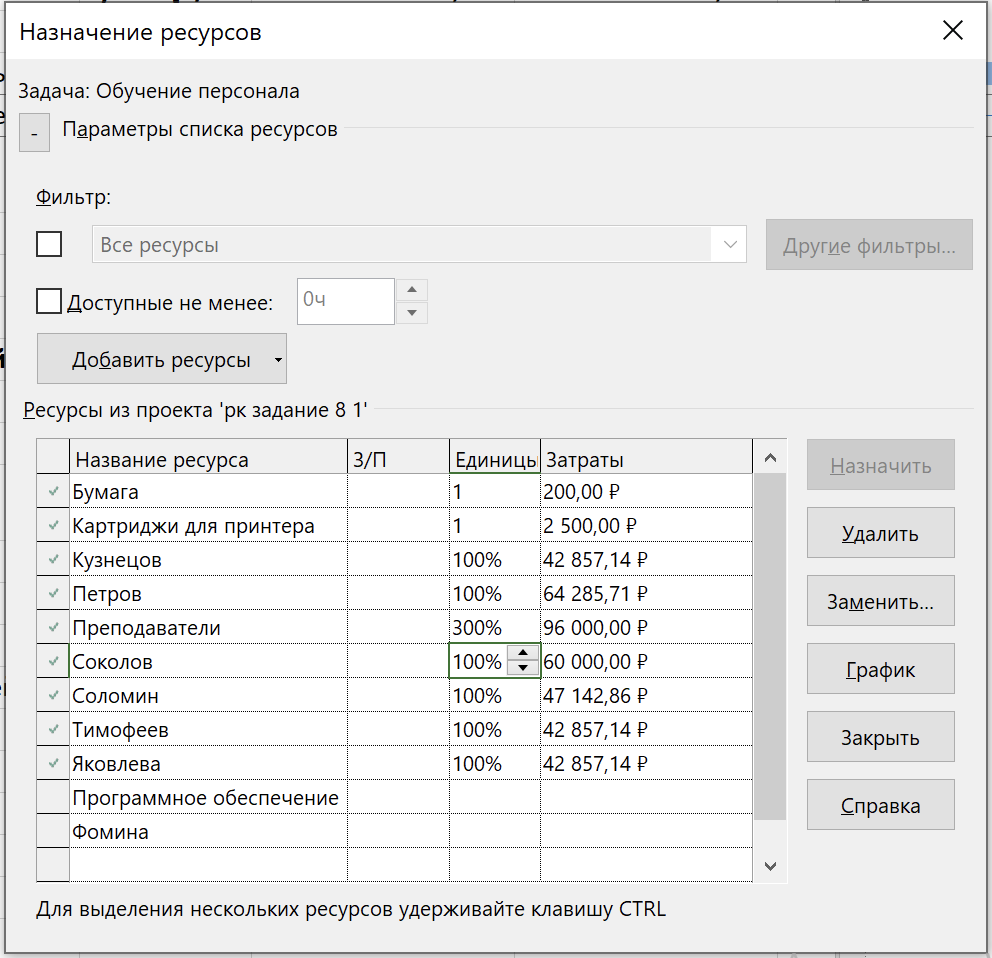
\includegraphics[scale=0.6]{11}
\end{figure}

Далее необходимо сравнить.

Поставить Соколова на задачу после того, как он завершит работы по установке программного обеспечения.

\begin{figure}[H]
  \centering
  \caption{Ставим Соколова. }
  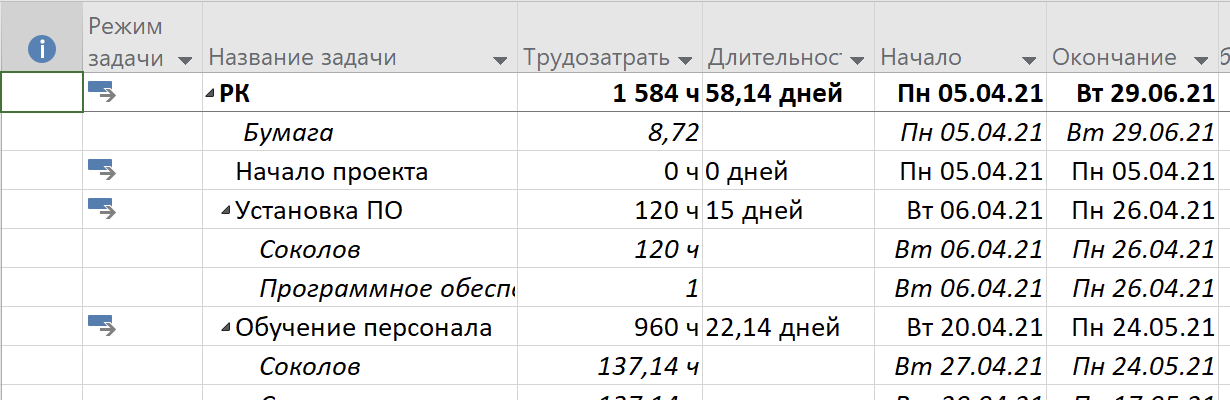
\includegraphics[scale=0.6]{12}
\end{figure}

В итоге сроки и бюджет проекта

\begin{figure}[H]
  \centering
  \caption{Сроки и бюджет. }
  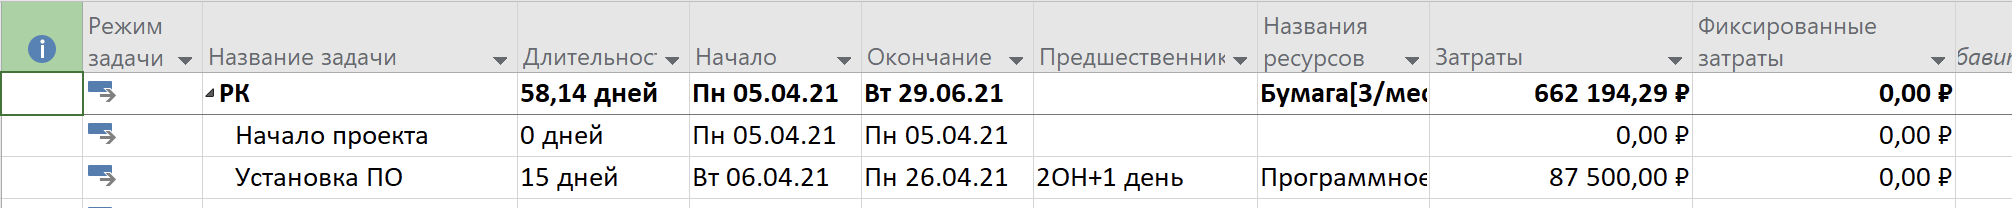
\includegraphics[scale=0.6]{13}
\end{figure}

Изменим профиль загрузки

\begin{figure}[H]
  \centering
  \caption{Ставим Соколова. }
  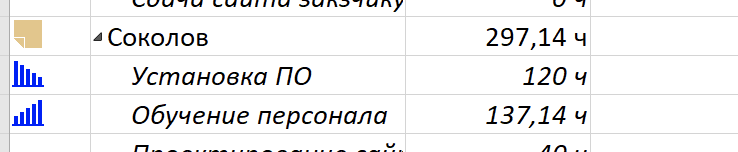
\includegraphics[scale=0.6]{14}
\end{figure}

В итоге сроки и бюджет проекта

\begin{figure}[H]
  \centering
  \caption{Сроки и бюджет. }
  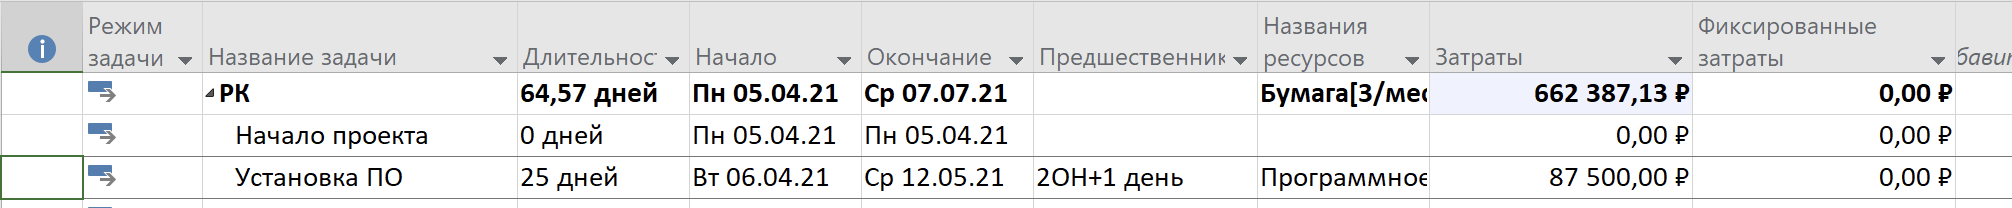
\includegraphics[scale=0.6]{15}
\end{figure}

В итоге затраты не поменялись, ведь сроки работ не изменились. Но после изменения профиля загрузки для Соколова, сроки выполнения общей задачи сдвинулись больше чем на неделю, значит далее продолжаем работать с первым изменением. Использование профиля не нужно.

\item \textbf{Задание 9}

Посмотрим критический путь проекта

\begin{figure}[H]
  \centering
  \caption{Критический путь. }
  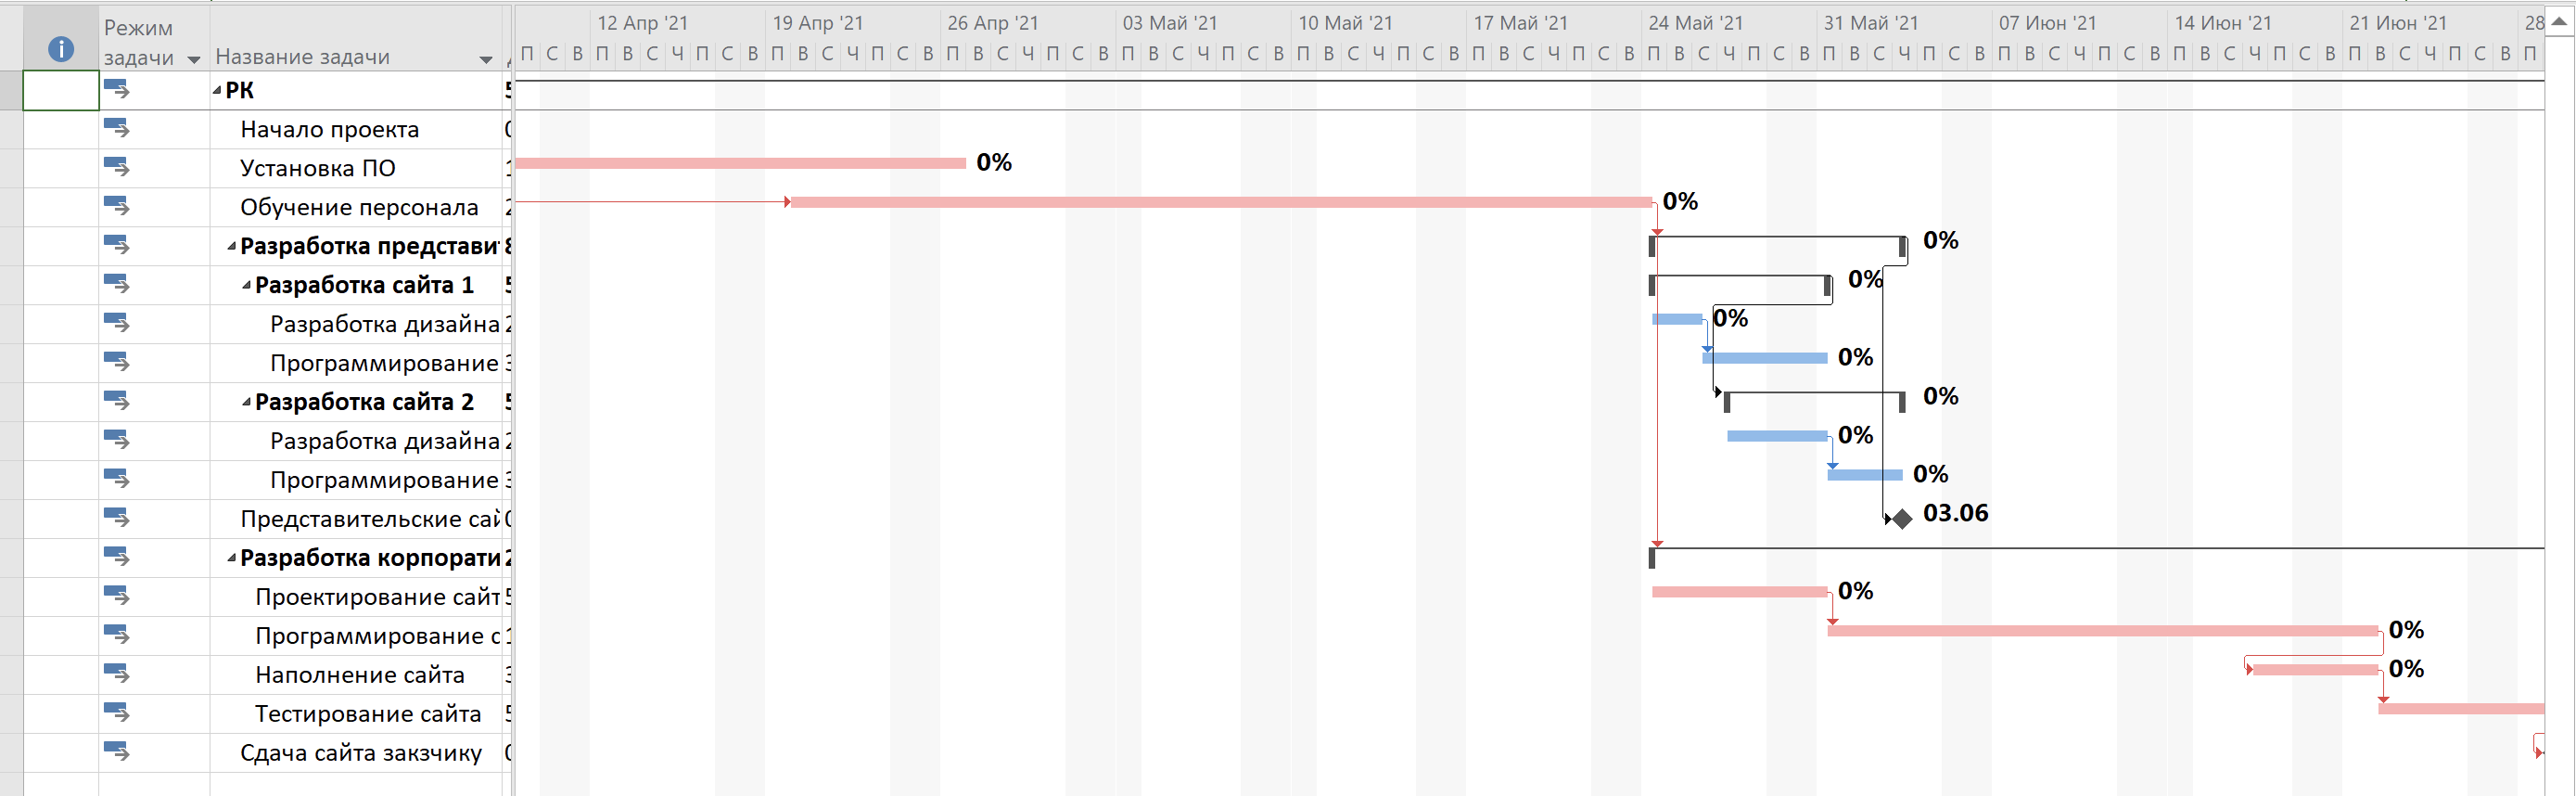
\includegraphics[scale=0.4]{16}
\end{figure}

Обучение мы сократить не можем. 

Программирование сайта является следующей из продолжительных в критическом пути и на неё можно добавить ещё одного программиста-стажера Иванова. Также добавим его на тестирование и проектирование. 

\begin{figure}[H]
  \centering
  \caption{Добавили стажера }
  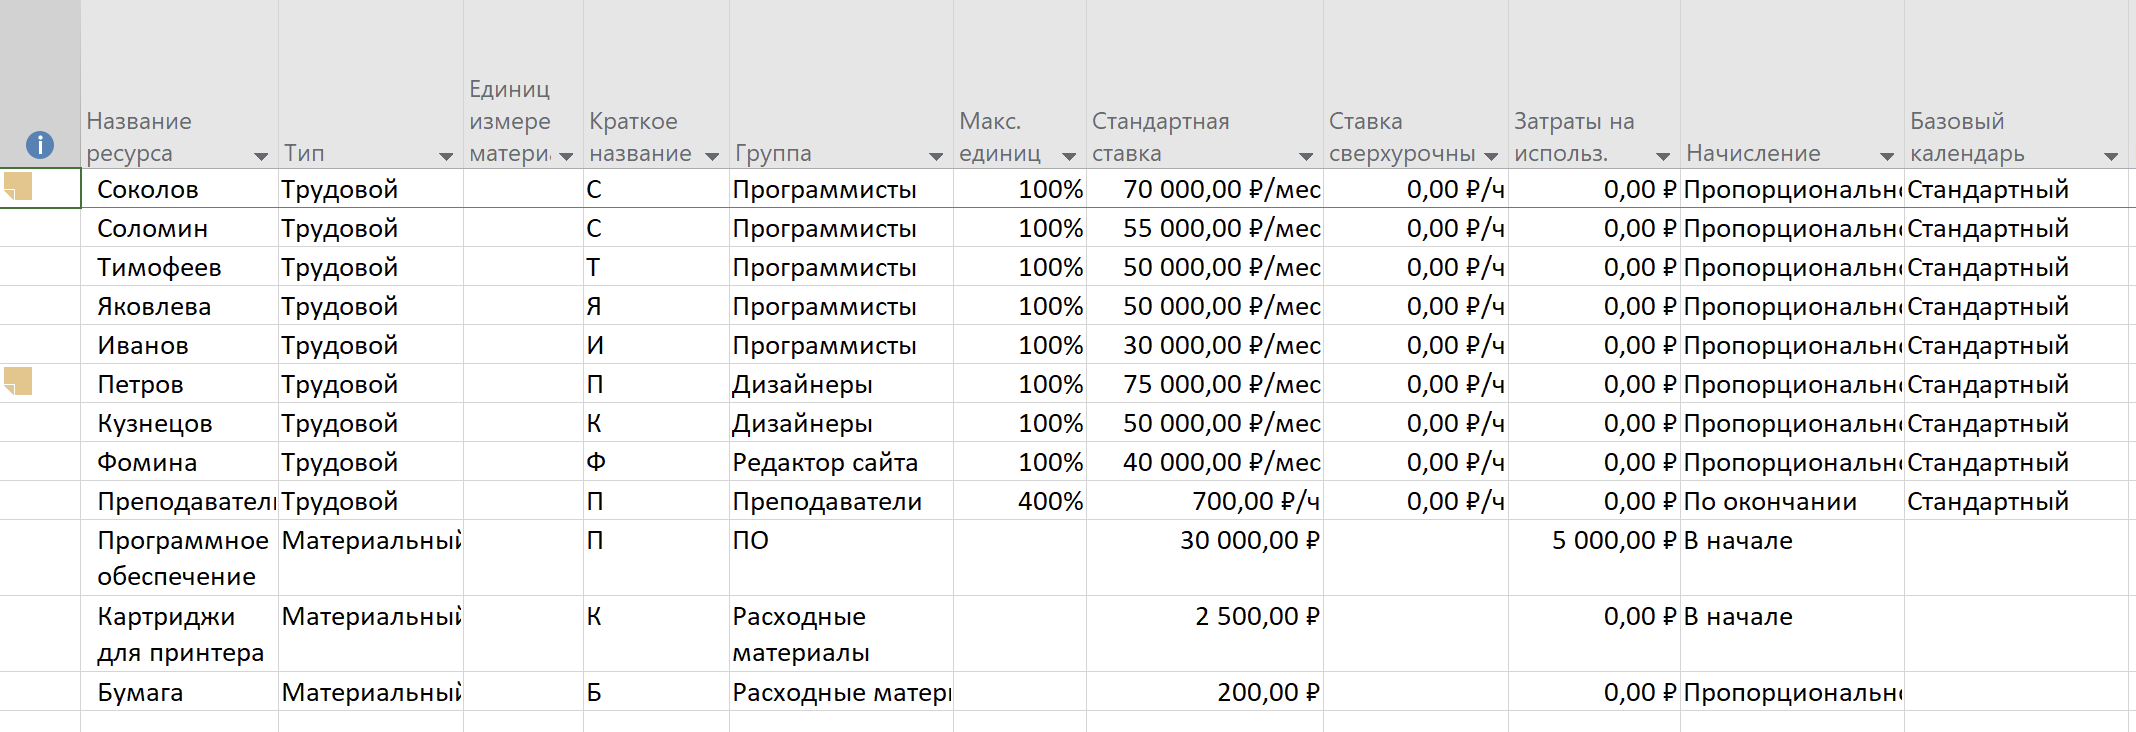
\includegraphics[scale=0.5]{17}
\end{figure}

\begin{figure}[H]
  \centering
  \caption{Итог }
  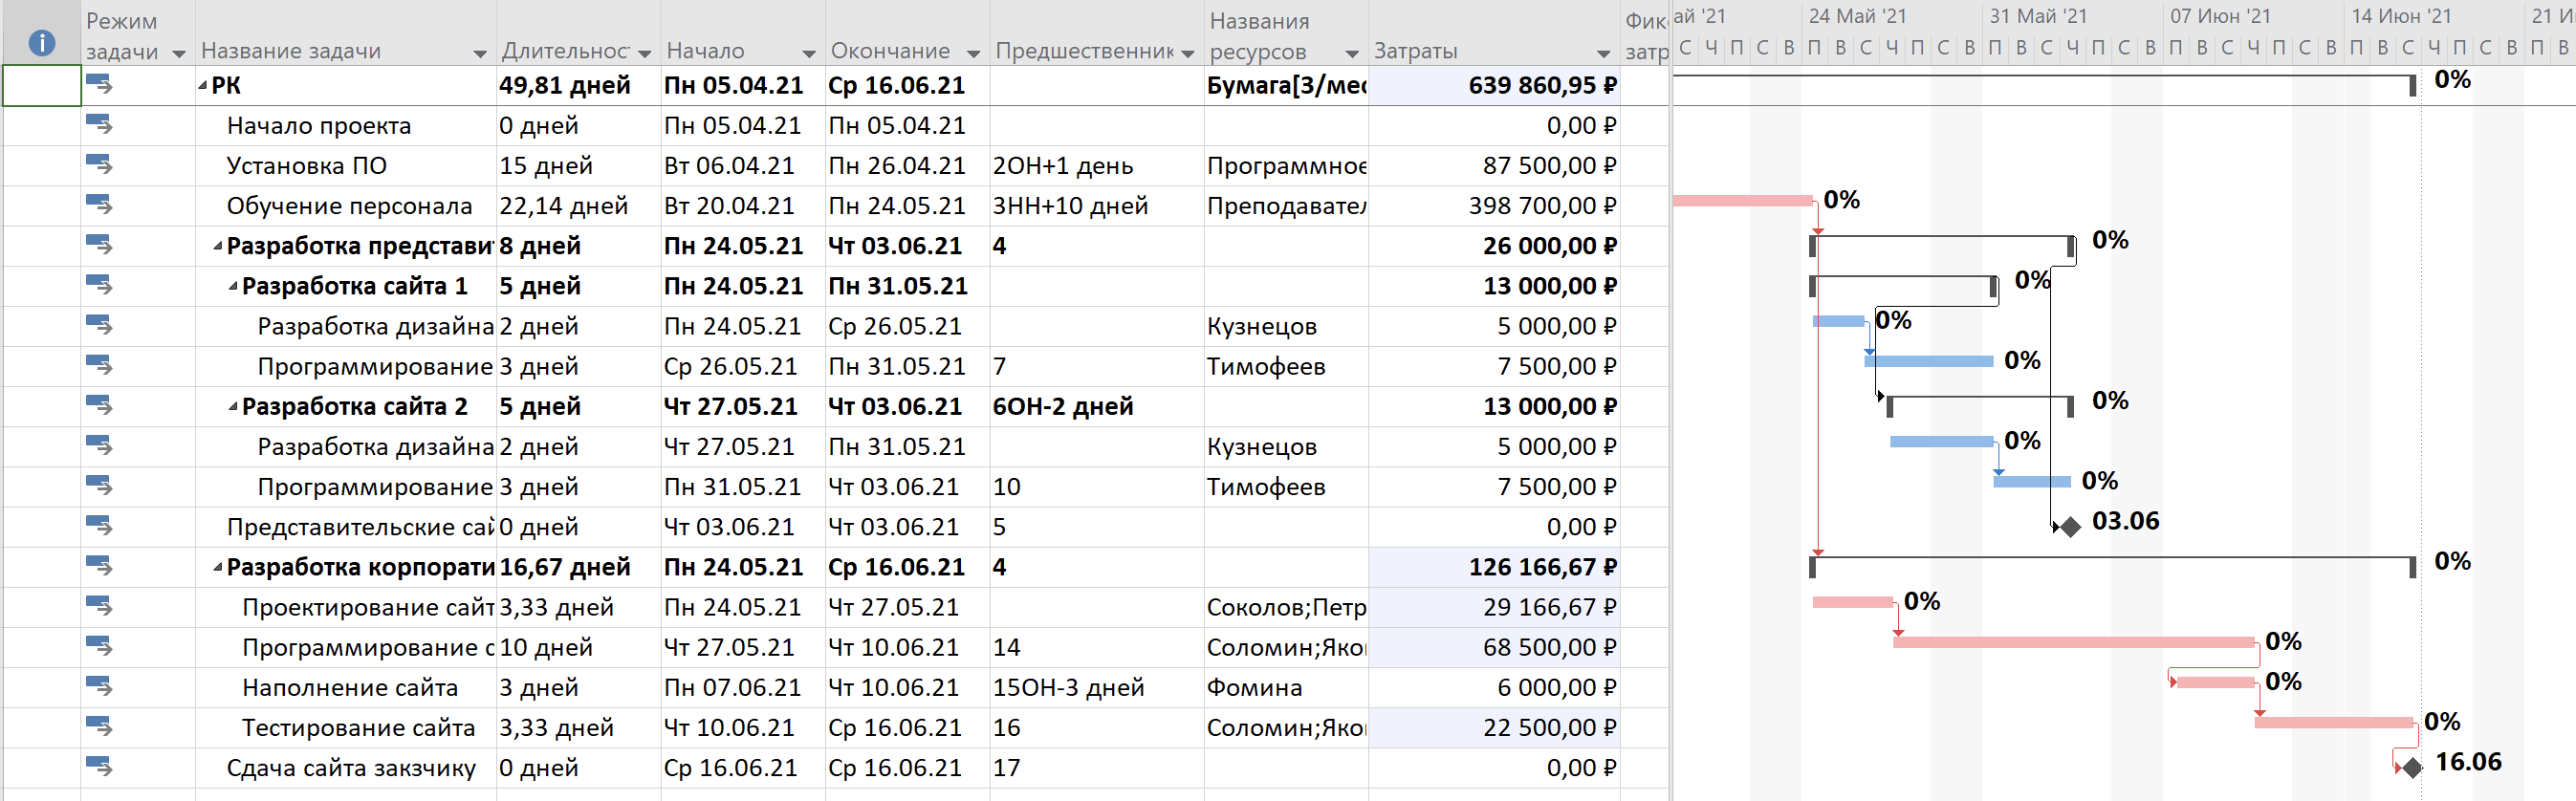
\includegraphics[scale=0.5]{18}
\end{figure}

Получилось сократить длительность проекта на 2 недели, а затраты на 22334 рублей.

Сохраняем базовый план проекта

\begin{figure}[H]
  \centering
  \caption{Базовый план }
  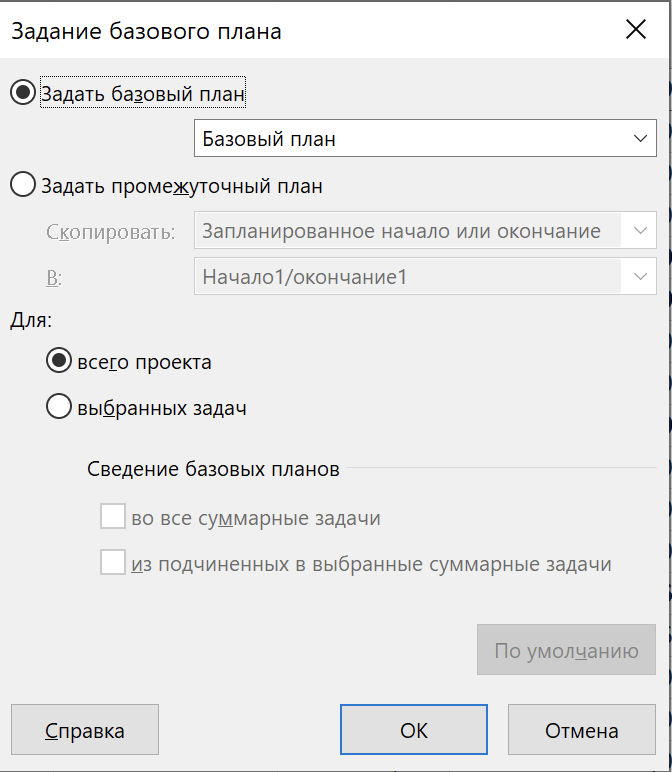
\includegraphics[scale=0.7]{19}
\end{figure}

\item \textbf{Задание 10}

Задаем дату отчета

\begin{figure}[H]
  \centering
  \caption{Дата отчета. }
  
\includegraphics[scale=0.7]{20}
\end{figure}

Далее задаем различную информацию о проекте.

Программирование сайта началось на 4 дня позже.

\begin{figure}[H]
  \centering
  \caption{Программирование сайта. }
  
\includegraphics[scale=0.7]{21}
\end{figure}

Разработка дизайна сайта задержалась на 2 дня.

\begin{figure}[H]
  \centering
  \caption{Разработка дизайна сайта. }
  
\includegraphics[scale=0.7]{22}
\end{figure}

С 1 мая поставщик решил поднять стоимость бумаги на 20\%.

\begin{figure}[H]
  \centering
  \caption{Дата отчета. }
  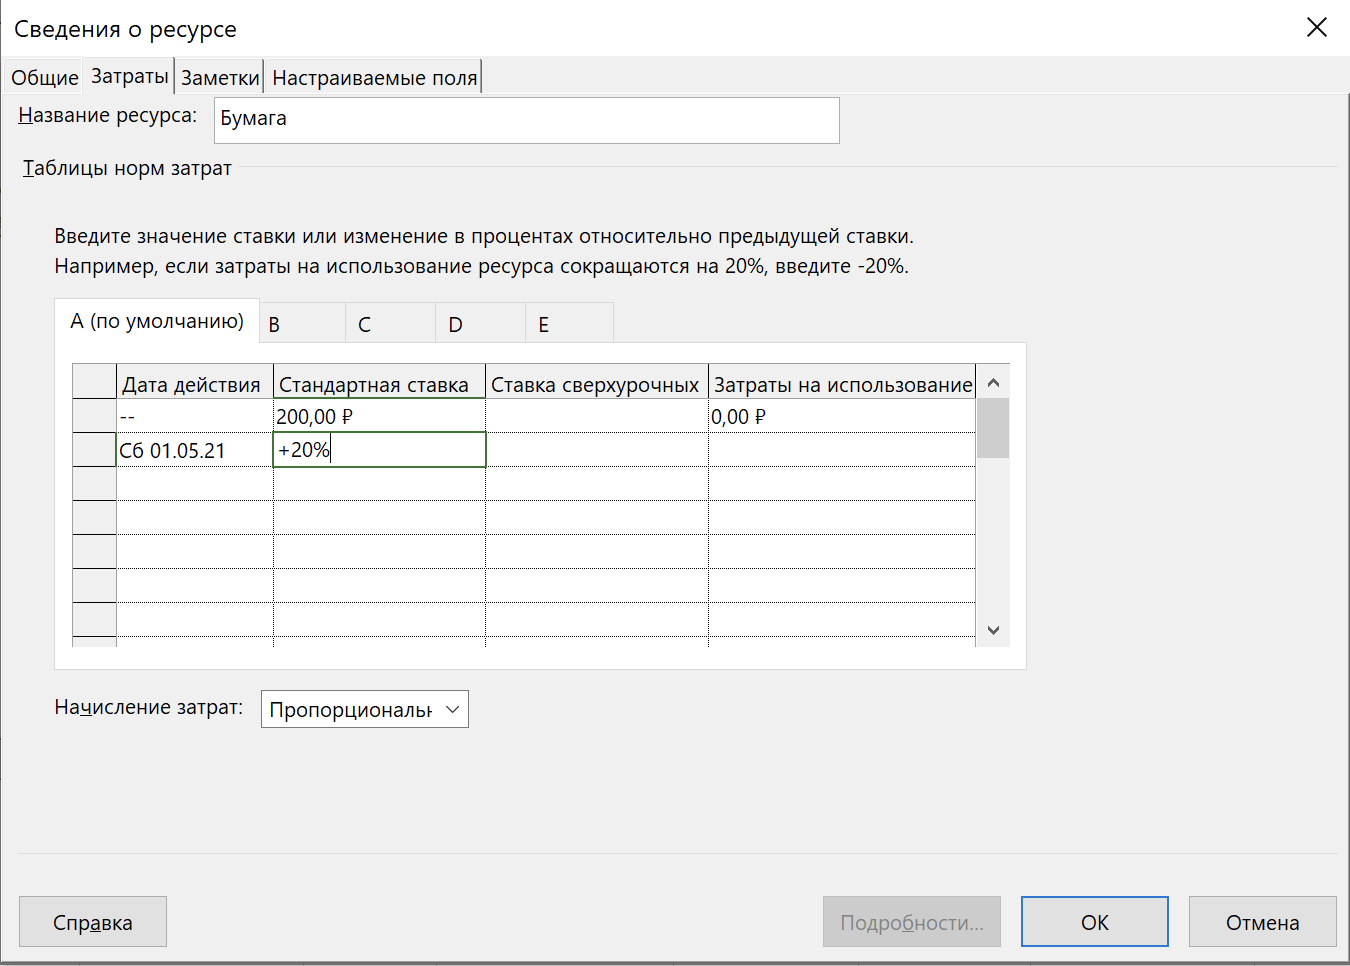
\includegraphics[scale=0.7]{23}
\end{figure}

С 1 мая преподаватели попросили надбавку в10\%, всвязи со сложностями в преподавании.

\begin{figure}[H]
  \centering
  \caption{Дата отчета. }
  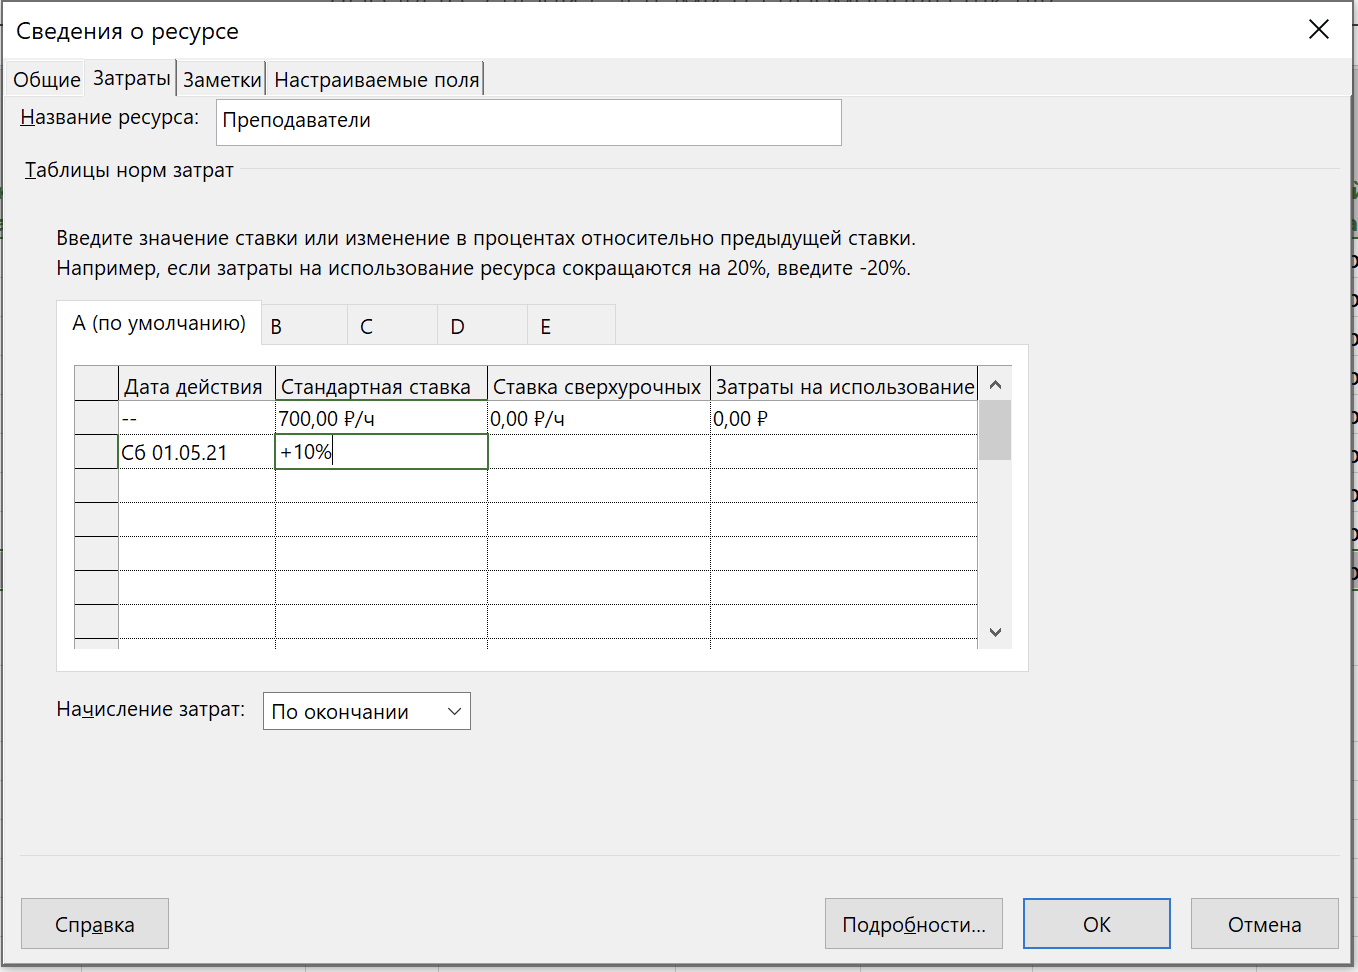
\includegraphics[scale=0.7]{24}
\end{figure}

Итого получается

\begin{figure}[H]
  \centering
  \caption{Итог. }
  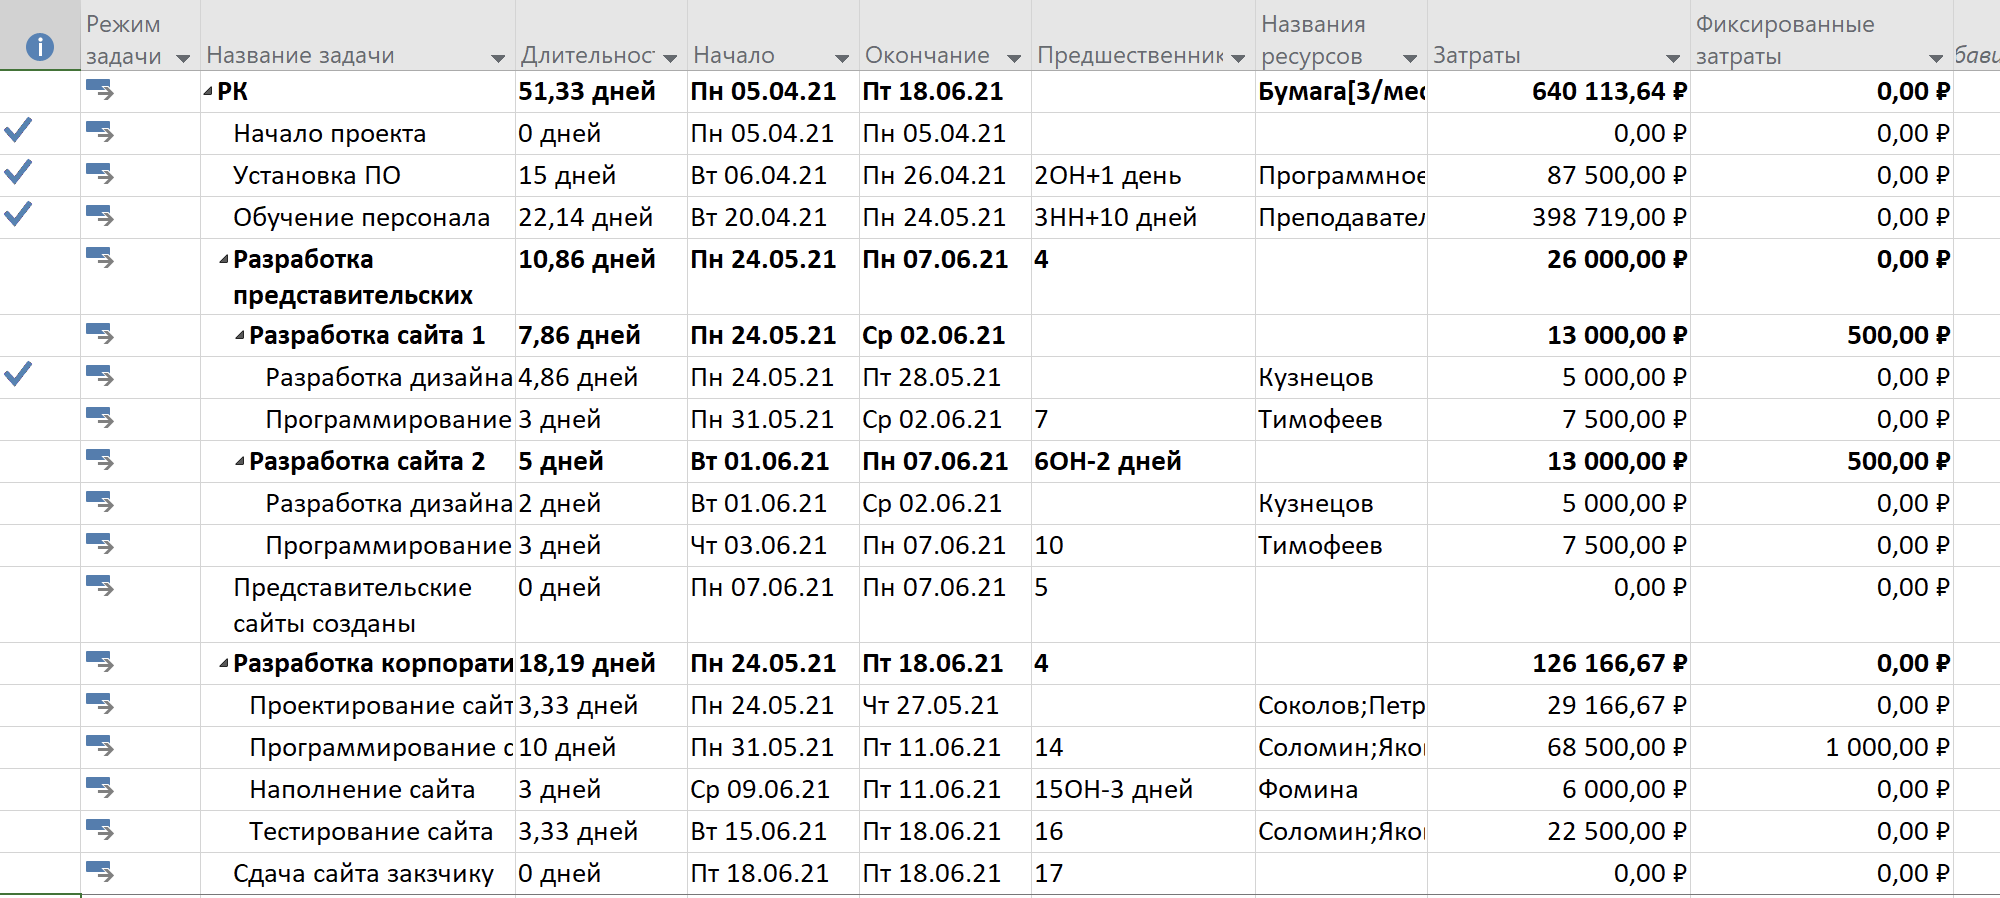
\includegraphics[scale=0.5]{25}
\end{figure}

Посмотрим отклонение от базового плана, выведя линию прогресса

\begin{figure}[H]
  \centering
  \caption{Линия прогресса. }
  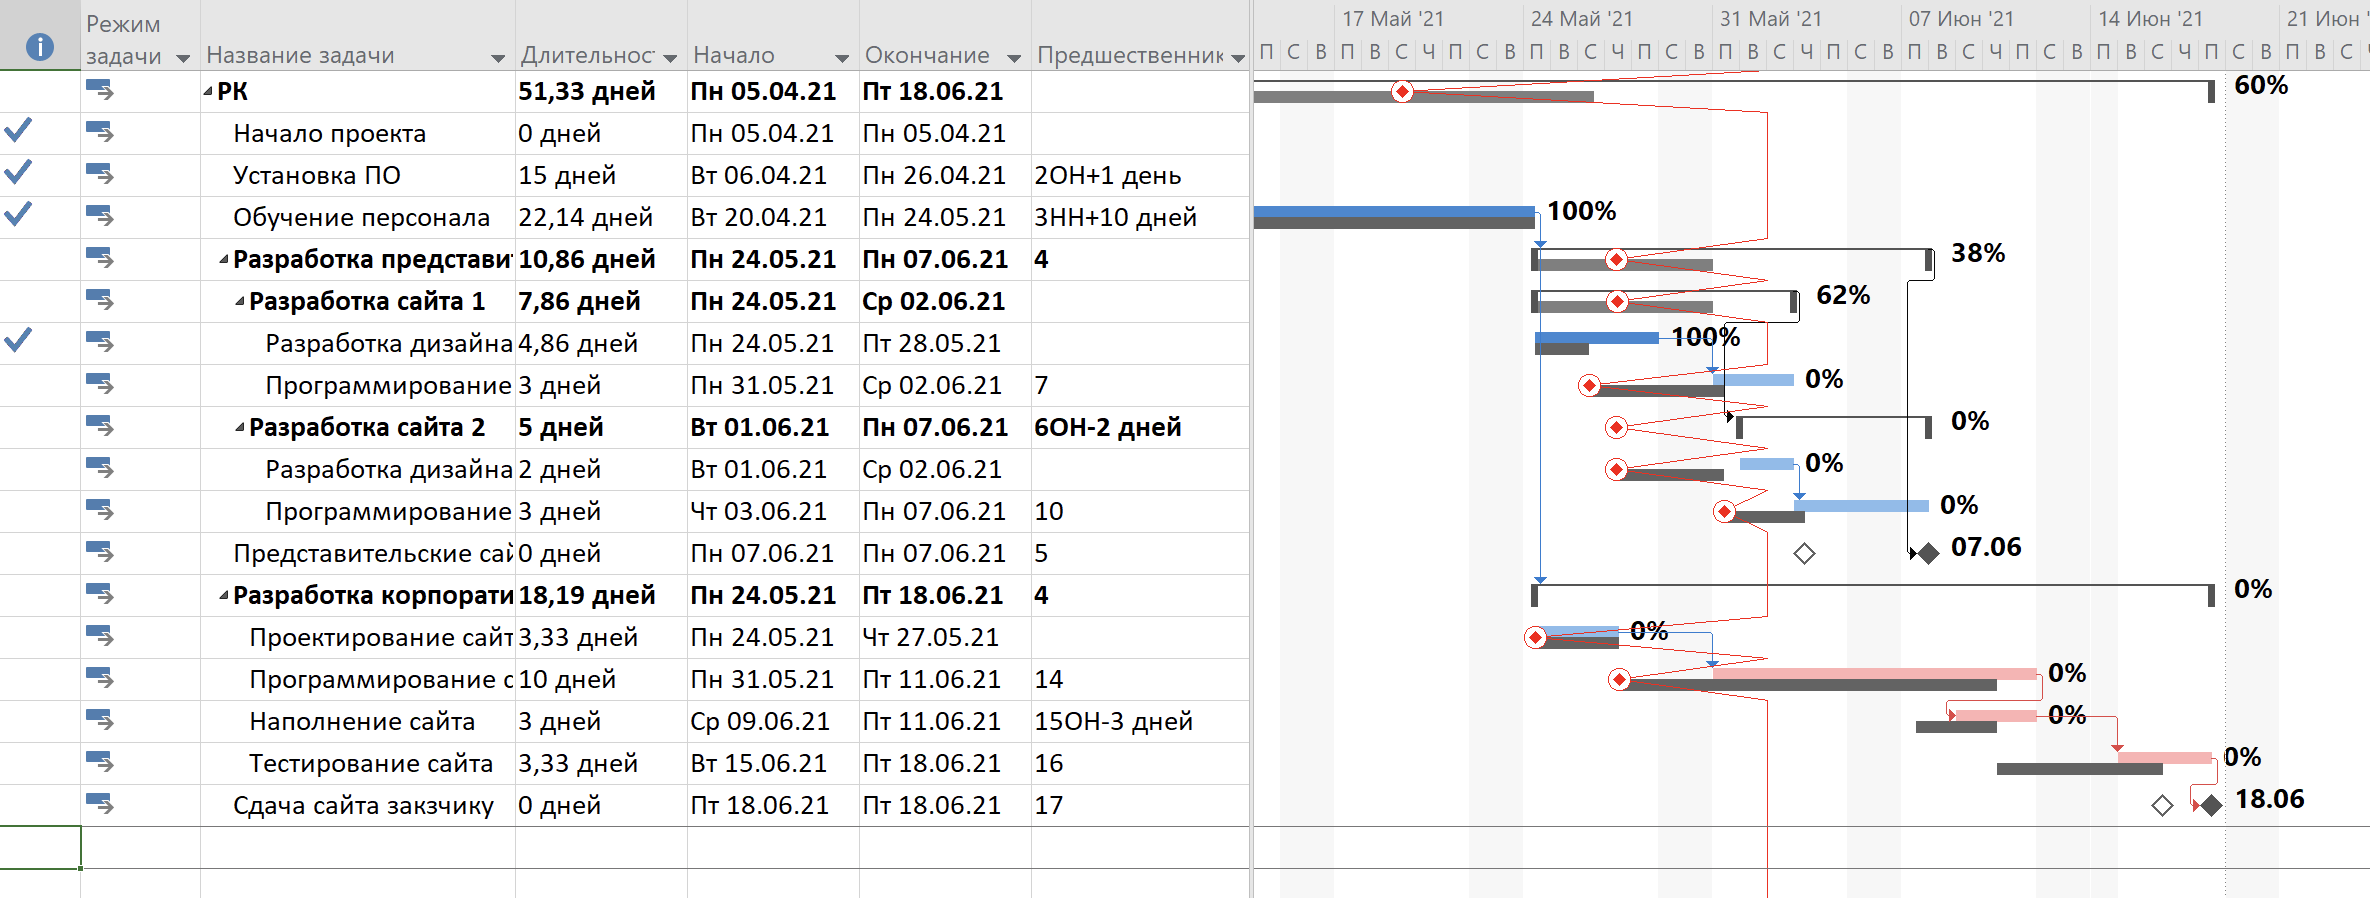
\includegraphics[scale=0.5]{26}
\end{figure}

Длительность проекта увеличилась на 2 дня, а сроки на 300 рублей.

Стоимостные параметры.

\begin{figure}[H]
  \centering
  \caption{Стоимостные парметры. }
  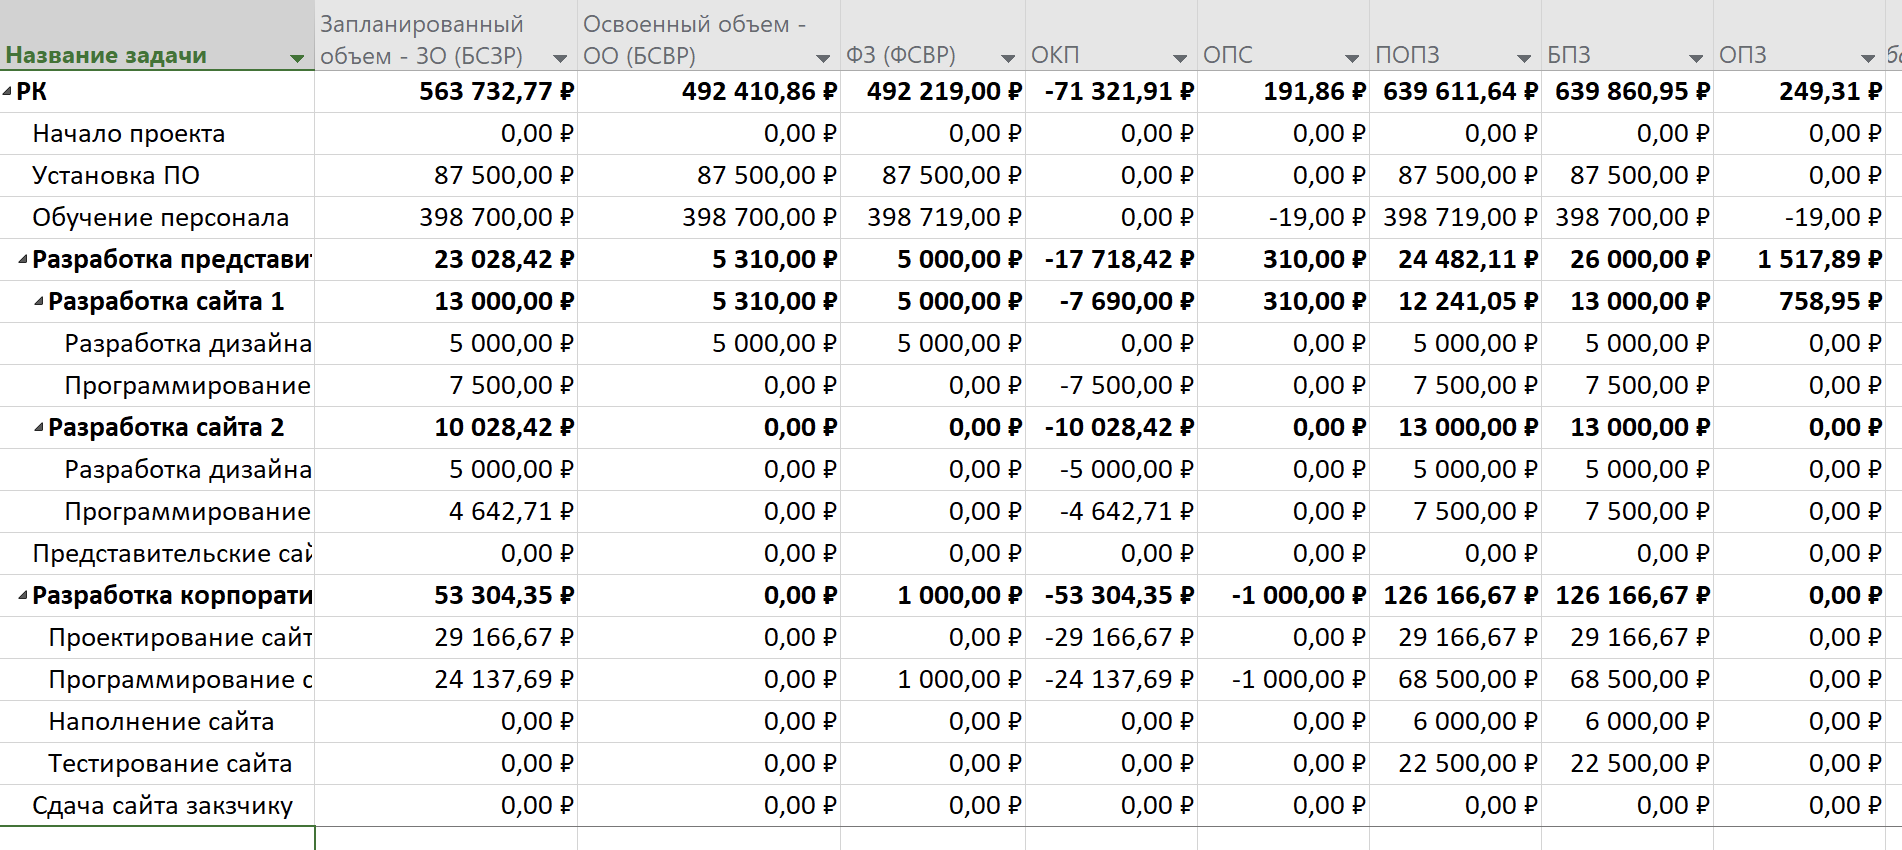
\includegraphics[scale=0.5]{27}
\end{figure}

Тогда

\textbf{Запланированный объем (ЗО)} -- средства, которые были бы затрачены на выполнение задачи в период с начала проекта до выбранной даты отчета, если бы задача точно соответствовала графику и смете. В нашем проекте: 563732 рублей.

\textbf{Базовая стоимость выполненных работ (БСВР)}-- средства, которые были бы затрачены на выполнение задачи с самого начала проекта до выбранной даты отчета, если бы фактически выполненная работа оплачивалась согласно смете. В нашем проекте: 492410 рублей (отклонение от базовой стоимости запланированных работ - 71321 рублей).

\textbf{Фактические затраты или фактическая стоимость выполненных работ (ФСВР)}-- средства, фактически потраченные на выполнение задачи в период с начала проекта до выбранной даты отчета. В случае проекта: 492219 рублей (отклонение от базовой стоимости выполненных работ 191 рубль). 

\textbf{Предварительная оценка по завершении (ПОПЗ)} -- ожидаемые общие затраты для задачи, расчет которых основан на предположении, что оставшаяся часть работы будет выполнена в точном соответствии со сметой. Для проекта: 639611 рублей.

Таким образом, на дату отчёта все идет по плану и укладываемся в срок и в финансы.

\end{enumerate}

\end{document}